%----------------------- Thesis Master Document -----------------------------------%
%                                                                                  %
% Hacked together by Thomas Griffiths 2014-01-08 tmg994(at)uowmail.edu.au          %
% If you get stuck read my comments here and in the preamble (thesispreamble.tex). %
% Hopefully they can help you find your answers will be I highly reccomend making  %
% friends with Google and http://tex.stackexchange.com/, the truth is out there.   %
%                                                                                  %
%----------------------------------------------------------------------------------%

%------------------------ Preamble and bibliography resources
\documentclass[12pt,oneside]{book}
%--------------- UOW Thesis Preamble ----------------------------------------%
% Thomas Griffiths 2013-07-16 tmg994@uowmail.edu.au                          %
%                                                                            %
% I encourage you to read the documentation for each of the packages below,  %
% they contain instructions for implementation and examples of their use.    %
% If you get stuck read my comments, hopefully they can help you find where  %
% your answers will be. I highly reccomend making friends with señor Google, %
% he knows quite a bit. The wikibook on LaTeX is also very helpful:          %
% http://en.wikibooks.org/wiki/LaTeX/                                        %
% The packages I've loaded here are the bare basics. and mainly deal with    %
% formatting, captions and things. There are thousands of packages out there %
% for all the disciplines and formatting you might need. Google what you're  %
% looking for and the keywords 'LaTeX' and 'package', You'll probably find   %
% what you're looking for. I encourage you to look on ctan, www.ctan.org/‎,   %
% for packages that might be relevant to your degree. If you're in science I % 
% can recomend the siunitx and the chemmachro (or mhchem) package. They make %
% it really easy to typeset chemical equations, any quantity with units and  %
% scientific notation.                                                       %
%                                                                            %
%----------------------------------------------------------------------------%

\usepackage{geometry}
	\geometry{a4paper,inner=4cm, outer=2cm, top=3cm, bottom=2cm}
	% Dimensions from UOW thesis guidelines.
	\pdfpagewidth=\paperwidth 
	\pdfpageheight=\paperheight
	% This acts as a failsafe to ensure things aren't stretched or moved when it's finally printed as a PDF.

%\usepackage[parfill]{parskip} 
% Activate to begin paragraphs with an empty (return) line, comment out the indent below if you chose the return line option.

\setlength{\parindent}{4ex}	% Sets the length of the paragraph indent. Current setup has a an indent. Disable this if you activate the return line above.

\usepackage{titlesec}

\setcounter{secnumdepth}{4}
\usepackage{amsmath}
	
\usepackage{setspace}
% Double or one and a half spacing.
	
\usepackage{graphicx}
	\DeclareGraphicsRule{.tif}{png}{.png}{`convert #1 `dirname #1`/`basename #1 .tif`.png}
% Graphics. Remove me and you won't have any figures, and that would be very boring.

\usepackage[usenames,dvipsnames,svgnames,table]{xcolor}
% Adds the ability to make coloured text and lines throughout the document. See documentation for xcolor.

%-------------------- Tables, figures and captions
\usepackage[font={small},labelfont={bf},margin=4ex]{caption}
% Makes bold labeled and smaller font captions. Must be loaded before the longtable package to avoid conflicts! 

\usepackage{longtable} 
% Long tables (more than one page). Different headers and footers for beginning and end pages, etc.

\usepackage{afterpage} 
% Make a longtable start on the next clear page, but fills the previous one with text first (no random gaps in the text-from long tables anymore! Man, the day I discovered this...)

\usepackage{booktabs} 
% Nice looking tables and lines in tables

\usepackage{multirow} 
% Entries in tables over multiple rows

\usepackage{lscape} 
% Pages in landscape

\usepackage{pdflscape} 
% Landscape pages also rotated in the pdf

\usepackage{wrapfig} 
% Allows figures that don't take up the entire width of the page, wrapping the text around the figure

%\usepackage[position=top,singlelinecheck=false,captionskip=4pt]{subfig} 
% Multiple figures in an individual figure. Fig. 1 a, b, c, etc. each with, or without, it's own individual caption, and with a global caption for all sub figures.

%-------------------- Special symbols and fonts
\usepackage{amssymb} 
% Maths symbols

%-------------------- Document sections, headers, footers, and bibliography
\usepackage{fancyhdr}											
% for creating different headers and footers

%-------------------- Bibliography
\usepackage[backend=biber,articletitle=true,style=chem-rsc,doi=false]{biblatex}
% This is the package that lets you create a bibliography. I recommend reading the biblatex documentation to understand all the options i've specified here. BibLaTeX was created to replace BibTeX. It has lots of extra fields and options. I'm also using the biber backend here rather than the default, it copes with unicode and so can deal with accented characters easily.

% Currently this is set up to use RSC style references with article titles displayed.

% Traditionally you would use BibTeX, a special build of TeX, the newer biblatex package is a more powerful bibliograpy management tool for LaTeX. You can make multiple chapter based bibliographies, footnote bibliographes, sort your references by date, author, order cited, essentially by any bit of citation data you happen to have. You can also have a seperate library with a differnet format for say books and articles. Or if you're a PhD student, the thesis references and your publications.

%\usepackage[numbers,super,comma,sort&compress]{natbib}				
	%\setcitestyle{square}										
	% places citations in square brackets to helps to distinguish between powers and citations
%This is the old natbib package that meshes with bibtex (rather than using the newer biblatex). It's here mainly for legacy purposes. Try to shift to biblatex if you can, it is cleaner in it's implementation and creating a custom citation style is easier then with bibtex.

\usepackage[unicode=true,colorlinks=true,linkcolor=black,citecolor=black,urlcolor=black,breaklinks=true]{hyperref}
% The hyperref package allows you to have clickable links in your pdf. It also allows you to have the mailto link associated with your name. It can be  a bit finicky, so load it last.

%-------------------- Command renewals, New commands etc.
\renewcommand{\thefootnote}{\alph{footnote}}							
%letters for footnotes instead of numbers to avoid confusion with references.
 % this must be left as \input, \include is giving me a hard time here and only here.
\usepackage[]{uowthesistitlepage}
% Creates the title page in accordance with UOW guidelines, includes the definition of the extra fields in \maketitle
\addbibresource{your_bibliography.bib}

%------------------------ Main Document --------------------------
\begin{document}
    \onehalfspace
	
%-------------- Information For The Title Page
% Title page info (see uowthesistitlepage package)
    \title{Citation context based scientific article summarization} 

    \author{Aman Aniket}
    % Full name, and any degrees held.
    
    \date{November, 2015} 
    % Month Year, alternatively use the \today macro for Month dd, yyyy.
    
    \degree{Master of Science in Mathematics and Computing} 
    % Write it in full: e.g. Bachelor of Science Medicinal Chemistry Honours
    
 
    \supervisor[2]{Dr. Pawan Goyal \& Dr. Sourav Mukhopadhyay} 
    % The optional argument (default 1) in square brackets is the number of supervisors. In the Curly braces list your supervisor(s) seperated by commas.
    
    %\cosupervisor[1]{Dr. C. O. Supervisor}
    % The same as the supervisor command above. This command is optional.
    
    \school{Mathematics} 
    % e.g Chemistry

%-------------- Front Matter
    \frontmatter
    \maketitle
    \declaration
    % These \phantomsection are to ensure that the hyperref package hyperlinks to the correct page in the electronic pdf. If you turn hyperref off they don't do anything so they can just stay here.
\phantomsection\addcontentsline{toc}{chapter}{Abstract}
\chapter*{Abstract} % Starred chapter=chapter with no number.
Quickly moving to a new area of research is painful for researchers due to the vast amount of scientific literature in each field of study. One possible way to overcome this problem is to summarize a scientific
topic. Our goal is to effectively solve this problem by using bibliometric text mining and summarization techniques to generate summaries of scientific literature. It is a proven fact that we can use citations to produce automatically generated, readily consumable, technical extractive summaries.We generate extractive summaries of a set of Question Answering (QA) and
Dependency Parsing (DP) papers, their abstracts, and their citation sentences and show
that citations have unique information amenable to creating a summary. This work is built upon C-LexRank, a model for summarizing single scientific articles based on citations, which employs community detection and extracts salient information-rich sentences. The work focuses on improving the efficiency of the state-of-the-art C-LexRank algorithm by using new similarity measures, fine-tuning various modules of the algorithm for a better performance than the baseline. We introduce a host of new features namely Unigram similarity, Bigram similarity, Number of citations, Unigram similarity of Part-of-speech tags, Bigram Similarity of Part-of-speech tags, Bibilographic coupling metrics, Co-citation metrics, Title similiarity, Author Similarity \& Temporal similiarity. We introduce a concept of thresholding the edges of similarity graph in the community detection of C-LexRank to improve the performance.
    \chapter*{Acknowledgments}
I would like to express my sincere gratitude to my supervisors Professor Pawan Goyal of the Department of Computer Science and Engineering, IIT Kharagpur and Professor Sourav Mukhopadhyay of Department of Mathematics, IIT Kharagpur for the continuous support of my research, for their patience, motivation, and immense knowledge. Their guidance helped me in all the time of research and writing of this thesis.

Apart from my supervisors, I would like to thank Mayank Singh, a research scholar in the CNERG Group, IIT Kharagpur for his constant help and support during the course of the project. He patiently discussed all my doubts and suggestions and was key to the output of the project.

Above all, I would like to thank my family and friends for supporting me in all my endeavours.


%-------------- Table of contents
    \cleardoublepage
    \phantomsection \pdfbookmark[0]{Contents}{Contents} 
    \tableofcontents
    % These \phantomsection are to ensure that the hyperref package hyperlinks to the correct page in the electronic pdf. If you turn hyperref off they don't do anything so they can just stay here.

%-------------- Chapters
    \cleardoublepage
    \mainmatter
    \chapter{Introduction}
\section{Automatic Text Summarization}
Automatic summarization is the process of reducing a text document with a computer program in order to create a summary that retains the most important points of the original document. As the problem of information overload has grown, and as the quantity of data has increased, so has interest in automatic summarization. Technologies that can make a coherent summary take into account variables such as length, writing style and syntax. Automatic data summarization is a very important area within machine learning and data mining. Summarization technologies are used today, in a large number of sectors in industry today. An example of the use of summarization technology is search engines such as Google. Other examples include document summarization, image collection summarization and video summarization. The main idea of summarization is to find a representative subset of the data, which contains the information of the entire set. Document summarization, tries to automatically create a representative summary or abstract of the entire document, by finding the most informative sentences. Similarly, in image summarization the system finds the most representative and important (or salient) images. Similarly, in consumer videos one would want to remove the boring or repetitive scenes, and extract out a much shorter and concise version of the video. This is also important, say for surveillance videos, where one might want to extract out only important events in the recorded video, since most of the events are uninteresting with nothing going on.
\pagebreak

\subsection{Extraction-based Summarization}

In this summarization task, the automatic system extracts objects from the entire collection, without modifying the objects themselves. Examples of this include keyphrase extraction, where the goal is to select individual words or phrases to "tag" a document, and document summarization, where the goal is to select whole sentences (without modifying them) to create a short paragraph summary. Similarly, in image collection summarization, the system extracts images from the collection without modifying the images themselves.

\subsection{Abstraction-based Summarization}
Extraction techniques merely copy the information deemed most important by the system to the summary (for example, key clauses, sentences or paragraphs), while abstraction involves paraphrasing sections of the source document. In general, abstraction can condense a text more strongly than extraction, but the programs that can do this are harder to develop as they require the use of natural language generation technology, which itself is a growing field.

While some work has been done in abstractive summarization (creating an abstract synopsis like that of a human), the majority of summarization systems are extractive (selecting a subset of sentences to place in a summary).

% \begin{figure}
% \centering
% 
\includegraphics[height=4cm]{figures/example.jpg}
% \caption[Chemistry cat.]{This is chemistry cat. Here he serves to demonstrate a figure in a LaTeX document, complete with caption. Notice his suave bow tie, but also that he has forgotten to label his solutions.}
% \end{figure}
\section{Citation Analysis}
Previous work has analyzed citation and collaboration networks (Teufel, Siddharthan, \& Tidhar, 2006; Newman, 2001) and scientific article summarization (Teufel \& Moens, 2002). Bradshaw (2002, 2003) benefited from citations to determine the content of articles and introduce “Reference Directed Indexing” to improve the results of a search engine. Nanba, Abekawa, Okumura, and Saito (2004) and Nanba et al. (2000) analyzed citation sentences and automatically categorize citations into three groups using 160 pre-defined phrase-based
rules. This categorization was then used to build a tool to help researchers analyze citations and write scientific summaries. Nanba and Okumura (1999) also discussed the same citation categorization to support a system for writing a survey. Nanba and Okumura (1999) and
Nanba et al. (2000) reported that co-citation implies similarity by showing that the textual similarity of co-cited papers is proportional to the proximity of their citations in the citing article.

Previous work has shown the importance of the citation sentences in understanding
scientific contributions. Elkiss et al. (2008) performed a large-scale study on citations and
their importance. They conducted several experiments on a set of 2, 497 articles from the
free PubMed Central (PMC) repository2 and 66 from ACM digital library. Results from this
experiment confirmed that the average cosine between sentences in the set of citations to an
article is consistently higher than that of its abstract. They also reported that this number
is much greater than the average cosine between citation sentences and a randomly chosen
document, as well as between citation sentences and the abstract. Finally, they concluded
that the content of citing sentences has much greater uniformity than the content of the
corresponding abstract, implying that citations are more focused and contain additional
information that does not appear in abstracts.

Nakov and Hearst (2012) performed a detailed manual study of citations in the area
of molecular interactions and found that the set of citations to a given target paper cover
most information found in the abstract of that article, as well as 20\% more concepts, mainly
related to experimental procedures.
Kupiec, Pedersen, and Chen (1995) used the abstracts of scientific articles as a target
summary. They used 188 Engineering Information summaries that are mostly indicative
in nature. Kan, Klavans, and McKeown (2002) used annotated bibliographies to cover
certain aspects of summarization and suggest guidelines that summaries should also include
metadata and critical document features as well as the prominent content-based features.
Siddharthan and Teufel (2007) described a new reference task and show high human
agreement as well as an improvement in the performance of argumentative zoning (Teufel,
2005). In argumentative zoning—a rhetorical classification task—seven classes (Own, Other,
Background, Textual, Aim, Basis, and Contrast) are used to label sentences according to
their role in the author’s argument.
The problem of automatic related work summarization is addressed by Hoang and Kan
(2010). In their work, Hoang and Kan used a set of keywords representing a hierarchy of
paper topics and assigned a score to each input sentence to construct an extractive summary.
Athar (2011) addressed the problem of identifying positive and negative sentiment polarity
in citations to scientific papers. Similarly, Athar and Teufel (2012) used context-enriched
citations to classify scientific sentiment towards a target paper.
    \chapter{Previous Work}
\section{C-LexRank Algorithm}
In this section we describe C-LexRank as a method to extract citing sentences that cover
a diverse set of factoids. The method works by modeling the set of citations as a network
of sentences and identifying communities of sentences that cover similar factoids. Once a
good division of sentences is made, we extract salient sentences from different communities.
Figure 1 illustrates a representative example that depicts C-LexRank$'$s process.

\begin{figure}[!htbp]
\centering
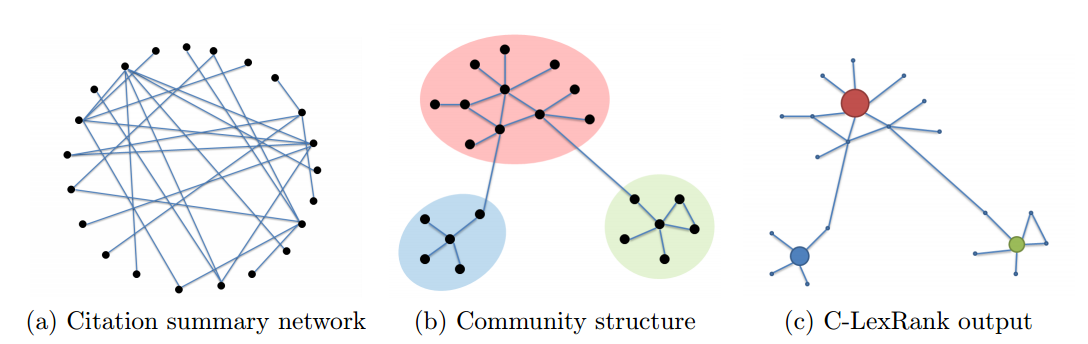
\includegraphics[width=15cm]{LexRank.png}
\caption{ The C-LexRank method extracts citing sentences that cover a diverse set of factoids.
The citation summary network in (a) models the set of sentences that cite
a specific paper, where vertices represent citing sentences and (weighted) edges
show the degree of semantic relatedness between vertex pairs. The community
structure in (b) corresponds to clustered sets of representative sentences extracted
from citation sentences. The C-LexRank output in (c) corresponds to the candidate
sentences from different clusters that are used for building a summary}
\label{cLexRank}
\end{figure}

\subsection{ Citation Summary Network}
In the first step (as shown in Figure 1 (a)), we model the set of sentences that cite a specific
paper with a network in which vertices represent citing sentences and undirected weighted
edges show the degree of semantic relatedness between vertex pairs, normally quantified
by a similarity measure. We refer to this network as the Citation Summary Network of
an article. The similarity function should ideally assign high scores to sentence pairs that
have the same factoids, and should assign low scores to sentences that talk about different
contributions of the target paper.
Previously, Qazvinian and Radev (2008) examined 7 different similarity measures including
TF-IDF with various IDF databases, longest common sub-sequence, generation
probability (Erkan, 2006), and the Levenstein distance on a training set of citations. They
showed that the cosine similarity measure that employs TF-IDF vectors assigns higher similarities
to pairs that contain the same factoids. Following Qazvinian and Radev (2008), we
use the cosine similarity between TF-IDF vector models that employ a general IDF corpus to construct the citation summary network of each article.

\begin{figure}[!htbp]
\centering
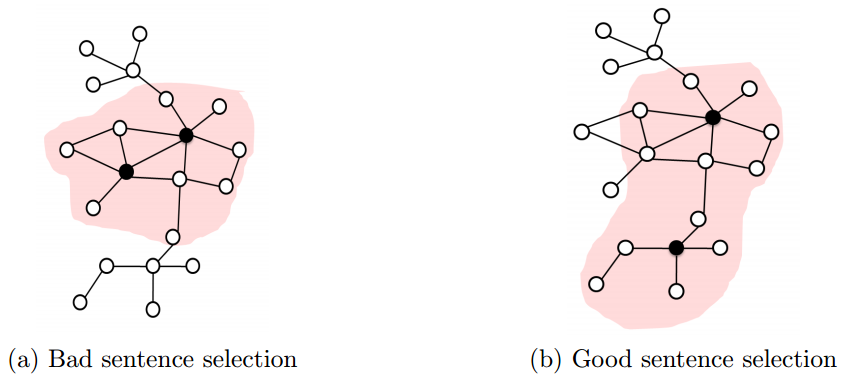
\includegraphics[width=15cm]{fig2lexrank.png}
\caption{ The C-LexRank method extracts citing sentences that cover a diverse set of factoids.
The citation summary network in (a) models the set of sentences that cite
a specific paper, where vertices represent citing sentences and (weighted) edges
show the degree of semantic relatedness between vertex pairs. The community
structure in (b) corresponds to clustered sets of representative sentences extracted
from citation sentences. The C-LexRank output in (c) corresponds to the candidate
sentences from different clusters that are used for building a summary}
\label{cLexRank2}
\end{figure}

\subsection{Community Structure}
In the second step (as shown in Figure 1 (b)), we extract vertex communities from the
citation summary network to generate summaries. We generate summaries by extracting
representative sentences from the citation summary network. Intuitively, a good summary
should include sentences that represent different contributions of a paper. Therefore, a good
sentence selection from the citation summary network will include vertices that are similar
to many other vertices and which are not very similar to each other. On the other hand,
a bad selection would include sentences that are only representing a small set of vertices
in the graph. This is very similar to the concept of maximizing social influence in social
networks (Kempe, Kleinberg, \& Eva Tardos, 2003). Figure 2 shows an example in which the ´
selected two vertices in the citation summary networks represent a small subset of vertices
(left) and a larger subset of vertices (right). In our work we try to select vertices that maximize the size of the set of vertices that they represent. We achieve this by detecting
different vertex communities in the citation summary network. In order to find vertex communities and thus a good sentence selection, we exploit the
small-world property of citation summary networks. A network is called \textit{small-world}, if
most of its vertices are not neighbors of each other, but can be reached from one another
by a small number of steps (Watts \& Strogatz, 1998). Recent research has shown that a
wide range of natural graphs such as biological networks (Ravasz, Somera, Mongru, Oltvai,
\& Barab´asi, 2002), food webs (Montoya \& Sol´e, 2002), brain neurons (Bassett \& Bullmore,
2006) and human languages (Ferrer i Cancho \& Sol´e, 2001) exhibit the small-world property.
This common characteristic can be detected using two basic statistical properties: the
clustering coefficient C, and the average shortest path length \textit{l}. The clustering coefficient
of a graph measures the number of closed triangles in the graph. It describes how likely
it is that two neighbors of a vertex are connected (Newman, 2003). Watts and Strogatz
(1998) define the clustering coefficient as the average of the local clustering values for each
vertex.
\begin{center}
C = $\frac{\sum_{i=1}^{n} c_i}{n}$
\end{center}


The local clustering coefficient $C_i$ for the $i_{th}$ vertex is the number of triangles connected
to vertex i divided by the total possible number of triangles connected to vertex i. Watts
and Strogatz (1998) show that small-world networks are highly clustered and obtain relatively
short paths (i.e., \textit{l} is small). Previous work (Qazvinian \& Radev, 2011a) shows that
citation summary networks are highly clustered. These networks have small shortest paths
and obtain clustering coefficient values that are significantly larger than random networks.
Moreover, Qazvinian and Radev suggest that this is because of a community structure, where each community is composed of a set of highly connected vertices with a small number
of edges that fall between communities.

\begin{figure}[!htbp]
\centering
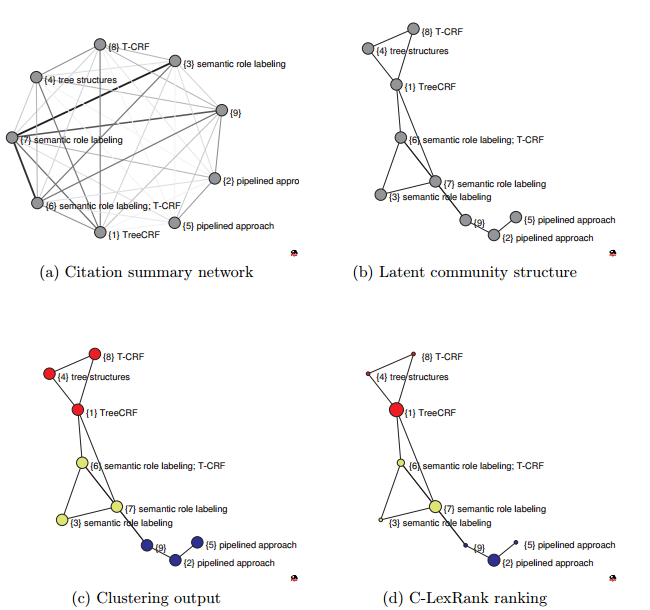
\includegraphics[width=15cm]{fig3lexRank.png}
\caption{ The C-LexRank method extracts citing sentences that cover a diverse set of factoids.
The citation summary network in (a) models the set of sentences that cite
a specific paper, where vertices represent citing sentences and (weighted) edges
show the degree of semantic relatedness between vertex pairs. The community
structure in (b) corresponds to clustered sets of representative sentences extracted
from citation sentences. The C-LexRank output in (c) corresponds to the candidate
sentences from different clusters that are used for building a summary}
\label{cLexRank}
\end{figure}


\subsection{Ranking}

The third step of the C-LexRank process (as shown in Figure 1 (c)) is applied after the
graph is clustered and the communities are formed. To produce the C-LexRank output,we extract sentences from different clusters to build a summary. We start with the largest
cluster and extract sentences using LexRank (Erkan \& Radev, 2004) within each cluster. In
other words, for each cluster Ωi we made a lexical network of the sentences in that cluster
(Ni). Using LexRank we can find the most central sentences in Ni as salient sentences of Ωi
to include in the main summary. We choose, for each cluster Ωi, the most salient sentence
of Ωi, and if we have not reached the summary length limit, we do that for the second most
salient sentences of each cluster, and so on. The cluster selection is in order of decreasing
size. Figure 3 (d) shows Cohn and Blunsom’s (2005) citation summary network, in which
each vertex is plotted with a size proportional to its LexRank value within its cluster. This
figure shows how C-LexRank emphasizes on selecting a diverse set of sentences covering a
diverse set of factoids.
Previously, we mentioned that factoids with higher weights appear in a greater number
of sentences, and clustering aims to cluster such fact-sharing sentences in the same communities.
Thus, starting with the largest community is important to ensure that the system
summary first covers the factoids that are more frequently mentioned in other citation
sentences and thus are more important.
The last sentence in the example in Table 2 is as follows. “We use CRFs as our models
for both tasks (Cohn \& Blunsom, 2005).” This sentence shows that a citation may not
cover any contributions of the target paper. Such sentences are assigned by the community
detection algorithm in C-LexRank to clusters to which they are semantically most similar.
The intuition behind employing LexRank within each cluster is to try to avoid extracting
such sentences for the summary, since LexRank within a cluster enforces extracting the most
central sentence in that cluster. In order to verify this, we also try a variant of C-LexRank
in which we do not select sentences from clusters based on their salience in the cluster, but
rather in a round-robin fashion, in which all the sentences within a cluster are equally likely
to be selected. We call this variant C-RR.

\pagebreak
\section{Evaluation scheme}

To evaluate our system, we use the pyramid evaluation method (Nenkova \& Passonneau,
2004). Each factoid in the citations to a paper corresponds to a summary content unit
(SCU) in (Nenkova \& Passonneau, 2004).
The score given by the pyramid method for a summary is the ratio of the sum of the
weights of its factoids to the sum of the weights of an optimal summary. This score ranges
from 0 to 1, and high scores show the summary content contains more heavily weighted
factoids. If a factoid appears in more citation sentences than another factoid, it is more
important, and thus should be assigned a higher weight. To weight the factoids we build a
pyramid, and each factoid falls in a tier. Each tier shows the number of sentences a factoid
appears in. Thus, the number of tiers in the pyramid is equal to the citation summary size.
If a factoid appears in more sentences, it falls in a higher tier.

So, if the factoid $f_i$ appears $\lvert f_i \rvert$
 times in the citation summary it is assigned to the tier $T_{\lvert f i\rvert}$.
 
 The pyramid score formula that we use is computed as follows. Suppose the pyramid
has n tiers, $T_i$
, where tier $T_n$ on top and $T_1$ on the bottom. The weight of the factoids in
tier $T_i$ will be i (i.e. they appeared in i sentences). If $\lvert T_i
\rvert$ denotes the number of factoids in
tier $T_i$
, and $D_i$
is the number of factoids in the summary that appear in $T_i$
, then the total
factoid weight for the summary is as follows.

\begin{center}
    D = $\sum_{i=1}^{n} i \times D_i$
\end{center}

Additionally, the optimal pyramid score for a summary with X factoids, is

\begin{center}
\textit{Max} = $\sum_{i=j+1}^{n} i \times \lvert T \rvert  + j \times (X - \sum_{i=j+1}^{n}\lvert T \rvert)$
\end{center}
where $j = max_i(\sum_{t=1}^{n}\lvert T_t \rvert \geq X)$ ). Subsequently, the pyramid score for a summary is calculated
as follows.

\begin{center}
P = $\frac{D}{Max}$
\end{center}

    \chapter{Experiments}
\section{Data-set}
To conduct our experiments, we chose the data-set which was used by the authors of C-LexRank algorithm. The data-set consists of 
\begin{itemize}
\item citations to 25 highly cited papers from 5 different domains: Text Summarization, Question Answering, Machien Translation, Textual Entailment, and Dependency Parsing.
\item Each dataset has a \textquotedblleft *.txt\textquotedblright file that has 1 citation per line, and a \textquotedblleft*.ann\textquotedblright file that has lines of the following format: \{ fact id \} \{ tab \} \{ nugget \}
\item To detect which nuggets/facts a citation contains, one should perform basic string matching.
\item The data-set is available on \href{http://www-personal.umich.edu/~vahed/resources/single.tar.gz}{this} link.
\end{itemize}
Further in our analysis, we needed the complete data-set for computations of graph based features which is available at \href{http://clair.eecs.umich.edu/aan/index.php}{The Association Of Computational Linguistics Anthology Network
}
\section{Preparing a baseline}
To evalulate the experiments, we prepare a set of baseline methods for comparison. 
\begin{itemize}
\item We first prepare a random summary of approximately 100 words and calculate the evaluation score.
\item We consider the state-of-the-art C-LexRank as a baseline for this study and prepare a summary for the same.
\end{itemize}
\section{Pre-processing}
We perform a couple of pre-processing steps to sanitize the input sentences in the citation context for efficient computation of similarities. 
\begin{itemize}
\item The reference to the name of authors and the year of the published work is removed for the computation of lexical features. This ensures that these blocks of text do not add noise to the values. An example of such a reference is :

\textit{examples of using nlp and ie in question answering include shallow parsing} \texttt{[kupiec 1993] [srihari \& li 2000]},\textit{ deep parsing}  \texttt{[li et al 2002] [litkowski 1999] [voorhees 1999]}, \textit{and ie} \texttt{[abney et al 2000] [srihari \& li 2000]}. 

The sentence after the references were removed was :

\textit{examples of using nlp and ie in question answering include shallow parsing , deep parsing , and ie}. 

\item We performed stemming on the words of the citation context and compared the evaluated results coming to a conclusion that stemming was not increasing the efficiency of the task making us remove it.

\item The next level of pre-processing was the removal of stop-words. Stop words are natural language words which have very little meaning, such as \textquotedblleft and \textquotedblright, \textquotedblleft the \textquotedblright, \textquotedblleft a \textquotedblright, \textquotedblleft and \textquotedblright, and similar words. The removal of stopwords had a positive effect on the quality of summaries as expected.

\end{itemize}

\begin{table}[]
\centering
\label{my-label}
\begin{tabular}{l|l}
\hline
\textbf{Description} & \textbf{Pyramid score} \\ \hline
Random summary       & 0.4762367241         \\ \hline
C-LexRank            & 0.64386657           \\ \hline
\end{tabular}
\caption{Preparing a baseline on 100 words summaries}

\end{table}


\section{Computing Features}
The similarity metrics between all pairs of sentences in a citation context are of critical importance to the performance of the algorithm. Considering this fact, we first started conducting experiments on exploring new features to improve the method of accurately capturing the similarity between a set of sentences belonging to the citation context. The previous work was based on computing the cosine similarity of TF-IDF vectorizations of the Bag of Words of unigrams present in the sentences. We started computing new features with an intention to better capture the similarity of topic between a set of sentences. These experiments were conducted by modifying the similarity measures for the community detection and the LexRank algorithm while keeping all other parameters intact. We calculated features from broadly three set of categories which are explained in the next sections. We ensure that the similarity scores calculated are in the range [0, 1]

\subsection{Lexical Features}
The dictionary meaning of lexical is \textit{of or relating to the words or vocabulary of a language, especially as distinguished from its grammatical and syntactical aspects.} We computed the following features with the grammatical and syntactical aspects as the intuition.

For 2 sentences in the citation context S1, S2

\subsubsection{Unigram similarity as a bag of words}

Unigram similarity involves calculation of cosine similarity using TD-IDF vectorization of unigrams after removing stopwords (stopwords are removed using NLTK corpora)

\subsubsection{Bigram similarity as a bag of words}
Bigram similarity involves calculation of cosine  similarity using TD-IDF vectorization of bigrams without removing stopwords

\subsubsection{Number of citations}
The number of citations in sentences of the citation context can be compared and can tell us about how similar two sentences are. Mathematically,  \\
Sim($ S_1, S_2 $) = $\frac{min (C(S_1), C(S_2))}{max (C(S_1), C(S_2))} $\\
Where,\\ C($S_i$) = Number of out-citations in the sentence $S_i$

\subsubsection{Unigrams of Part-of-Speech Tags}
For 2 sentences in the citation context, we tag their parts of speech using a standard POS tagger available with the NLTK package and calculate the cosine similarity after TF-IDF vectorization of the POS tags for the 2 sentences.

\subsubsection{Unigrams of Part-of-Speech Tags}
For 2 sentences in the citation context, we tag their parts of speech using a standard POS tagger available with the NLTK package and calculate the cosine similarity after TF-IDF vectorization of bigrams of POS tags for the 2 sentences.

\subsection{Graph Based Features}

\subsubsection{Bibilographic Coupling} 
Two documents are bibliographically coupled if they both cite one or more documents in common. The "coupling strength" of two given documents is higher the more citations to other documents they share. We calculate the bibilographic coupling of the 2 sentences using the following formula \\ 

sim ($S_1, S_2$) = $\frac{\lvert intersection(outCites(S1), outCites(S2) \rvert} { min ( \lvert outCites(S_1) \rvert, \lvert outCites(S_2) \rvert )}$ \\
Where, \\

inCites($S_i$) = Out-vertices of $S_i$ in the citation graph \\
intersection(A, B) = set of common elements in A \& B and, \\
$\lvert A \rvert$ = cardinality of list A

\subsubsection{Co-citation} 
Co-citation, like Bibliographic Coupling, is a semantic similarity measure for documents that makes use of citation relationships. Co-citation is defined as the frequency with which two documents are cited together by other documents.[1] If at least one other document cites two documents in common these documents are said to be co-cited. The more co-citations two documents receive, the higher their co-citation strength, and the more likely they are semantically related. We calculate the co-citation metric of 2 sentences by \\

Sim ($S_1, S_2$) = $ \frac{ \lvert intersection(inCites(S_1), inCites(S_2) \rvert}{ min ( \lvert inCites(S1) \rvert, \lvert inCites(S2) \rvert )}$ \\
Where, \\
inCites($S_i$) = In-vertices of $S_i$ in the citation graph

\subsection{Miscellaneous Features}

\subsubsection{Title similarity}
We calculate the unigram-similarity of the titles of the two documents that the 2 sentences belong to,  trying to establish the similarity measure between the 2 sentences \\
Sim ($S_1, S_2$) = Unigram-Similarity(Title(paper1), Title(paper2))

\subsubsection{Author similarty} 
We calculate the similarity in the set of authors between the two citing papers using overlapping similarity \\ 
Sim ($S_1, S_2$) = $\frac{\lvert intersection(authors(S_1), authors(S_2) \rvert}{  min ( \lvert authors(S1)\rvert, \lvert authors(S2) \rvert ) }$ \\
Where, \\
authors($S_i$) = list of authors of $S_i$

\subsubsection{Time based similarity}  
Time based similarity tries to capture the intuition that works citing the target document in a brief period belong to the same topic thus increasing the similarity between them \\
Sim ($S_1, S_2$) = $max(0, \frac{(1 - abs(year1 - year2))}{5})$\\
Where,\\
abs (x) = absolute value of x\\
year1 = publication year of S1\\
year2 = publication year of S2\\


\section{Combining Features}
After the calculation of features individually, we devised an approach to combine their values to represent a single similarity score for a set of citation context sentences. We took a variety of approaches to compute this which we describe in this section.

\subsection{Feature scaling} \label{scaling}

Before combining scores of individual features, we normalized the individual scores from various features by using a feature scaling technique to ensure that the range becomes [0, 1] 

\subsection{Mean of similarities} \label{mean}
We initiated combining the features by calculating the mean of individual similarity scores for the five features which demonstrated the highest evaluation pyramid scores.

\subsection{Maximum of similarities} \label{max}
In this experiment, the maximum value among the similarity scores by the combination of features was taken as the similarity score for the set of sentences in the citation context. 

\subsection{Minimum of similarities} \label{min}
We observed the the minimum of similarities for the combination of features was providing us the best evaluation scores on the data-set. Thus, minimum of similarity metrics from individual features was chosen as the method to combine features and calculate the similarity scores.


\section{Defining threshold for community detection}\label{thres}

To ensure that the resultant similarity weighted graph in the community detection module of the algorithm consists of relevant similarities and does not contain noise, we set up a threshold $ \alpha \in $ [0, 1] for the selection of edges in the community detection network. For a threshold $ \alpha $, we select top 100 edges in a list sorted by descending order of similarities. A default cut-off of 0.1 is taken for the similarity scores of the LexRank module of the algorithm.
    \chapter{Results \& Discussion}
\section{Results}

The following table summarizes results for all the experiments performed. For a detailed description of experiments, please refer to Chapter 3. The initial experiments on combining features were performed without feature scaling ( refer to \ref{scaling} for details). \ref{result1} shows the results of the experiments

\begin{itemize}
\item \texttt{Mean()} is calculated as described in \ref{mean}
\item \texttt{Max()} is calculated as described in \ref{max}
\item \texttt{Min()} is calculated as described in \ref{min}
\item The value of $ \alpha $ is the threshold which is discussed in \ref{thres}
\end{itemize} 

The list of features used in the experiment are as follows :

\begin{table}[!htbp]
\centering
\begin{tabular}{l|l|l}
\hline
\textbf{Index} & \textbf{Feature description}  & \textbf{Pyramid Score} \\ \hline
1              & Unigrams                      & 0.6658455015           \\ \hline
2              & Bigrams                       & 0.6212465025           \\ \hline
3              & No of citations               & 0.5800021814           \\ \hline
4              & UG of POS Tags                & 0.6512963561           \\ \hline
5              & BG of POS Tags                & 0.5258799947           \\ \hline
6              & Bibilographic coupling        & 0.5758991342           \\ \hline
7              & Co-citation matrix similarity & 0.4668755464           \\ \hline
8              & Title similarity              & 0.5743987379           \\ \hline
9              & Author similarity             & 0.5476835667           \\ \hline
10             & Time similarity               & 0.5583852299           \\ \hline
\end{tabular}
\caption{Feature indexes and pryramid scores for individual features}
\label{my-label}

\end{table}



\begin{table}[!htbp]
\centering
\begin{tabular}{l|l}
\textbf{Method description}                                  & \textbf{Pyramid score}                     \\ \hline
\multicolumn{1}{l|}{Mean({[}1,2,3,4,6{]}) (top 5)}          & \multicolumn{1}{l}{0.6173276955}          \\ \hline
\multicolumn{1}{l|}{Mean({[}1,4{]}) (top 2)}                & \multicolumn{1}{l}{0.6155651665}          \\ \hline
\multicolumn{1}{l|}{Mean({[}1:10{]})}                       & \multicolumn{1}{l}{0.6120720413}          \\ \hline
\multicolumn{1}{l|}{Mean ({[}1, 3, 4{]}) (top 3)}           & \multicolumn{1}{l}{0.641261796}           \\ \hline
\multicolumn{1}{l|}{Max {[}1,4,8{]}}                        & \multicolumn{1}{l}{0.5846927132}          \\ \hline
\multicolumn{1}{l|}{Max ({[}1,4,8{]}) ; $ \alpha $ = 0.8}   & \multicolumn{1}{l}{0.5658356889}          \\ \hline
\multicolumn{1}{l|}{Min ({[}1,4,8{]});  $ \alpha $ = 0.9}   & \multicolumn{1}{l}{0.5884321604}          \\ \hline
\multicolumn{1}{l|}{Min ({[}1,4,8{]}); $ \alpha $ = 0.8}    & \multicolumn{1}{l}{\textbf{0.6706331335}} \\ \hline
\multicolumn{1}{l|}{Min ({[}1,4,8{]}); $ \alpha $ = 0.95}   & \multicolumn{1}{l}{\textbf{0.6934690128}} \\ \hline
\multicolumn{1}{l|}{Min ({[}1,4,8{]}); $ \alpha $ = 0.85}   & \multicolumn{1}{l}{\textbf{0.7187605304}} \\ \hline
\multicolumn{1}{l|}{Min ({[}1,4,8{]}); $ \alpha $ = 0.9}    & \multicolumn{1}{l}{\textbf{0.7105636008}} \\ \hline
\multicolumn{1}{l|}{Min ({[}1,2,4,8{]}); $ \alpha $ = 0.85} & \multicolumn{1}{l}{0.6193834661}          \\ \hline
\multicolumn{1}{l|}{Min({[}1,2,4,8{]}); $ \alpha $ = 0.9}   & \multicolumn{1}{l}{0.5856727122}          \\ \hline
\multicolumn{1}{l|}{Min ({[}1,4,6,8{]}); $ \alpha $ = 0.85} & \multicolumn{1}{l}{\textbf{0.7228621087}} \\ \hline
\end{tabular}
\caption{Evaluation scores for feature combinations without feature scaling }
\label{result1}

\end{table}
\pagebreak
After we implement feature scaling we obtain the results as noted in \ref{result2}. The values in bold indicate that the corresponding experiment performed better than the baseline methods. The combination of [1,4,6,8] was chosen to keeping diversity of type of features and best individual pyramid scores in mind.\\[20pt]

\begin{table}[!htbp]
\centering
\begin{tabular}{l|l}
\hline
\textbf{Method description}              & \textbf{Pyramid score} \\ \hline
Min ({[}1,2,4,8{]}); $ \alpha $ = 0.85   & \textbf{0.679249946}   \\ \hline
Min ({[}1,2,4,6,8{]}); $ \alpha $ = 0.85 & 0.6286947577           \\ \hline
Min ({[}1,4,8{]}); $ \alpha $ = 0.85     & \textbf{0.6690628106}  \\ \hline
Min ({[}1,4,6,8{]}); $ \alpha $ = 0.85   & \textbf{0.7151122733}  \\ \hline
Min ({[}1,3,4,6,8{]}); $ \alpha $ = 0.85 & 0.6593057212           \\ \hline
Min ({[}1,4,6,8{]}); $ \alpha $ = 0.9    & \textbf{0.7053210946}  \\ \hline
\end{tabular}

\caption{Evaluation scores for feature combinations with feature scaling }
\label{result2}

\end{table} 
\pagebreak
\section{Discussion \& Future work}
\begin{itemize}
\item We introduce new features to capture the notion of similarity between a pair of sentences in the citation context which we prove produces better results than the state-of-the-art system.
\item We develop a method to combine multiple feature similarity scores to obtain a single score for a pair of sentences. 
\item We fine-tune C-LexRank's graph to improve community detection by introducing the notion of a threshold which gives us better results than the previous system.
\item However we may be dealing with a situation of over-fitting which we intend to cross-verify using a neutral corpus of scientific documents in future.
\item We may shift to a non-factoid based evaluation scheme in future to be able to test the algorithm on a much larger dataset.
\item We also intend to perform the summarization on biomedical scientific documents to better understand medical conditions through a summarized time-line of research and development in the particular field.

\end{itemize}
    \include{chapters/chap5}

%-------------- Bibliography
    \cleardoublepage
    \phantomsection	%\addcontentsline{toc}{chapter}{Bibliography}										
    %\printbibliography

%-------------- Appendicies
    \cleardoublepage
    \appendix
    \chapter{Appendix One}
\section{List of technologies used}
Following are the list of technologies used in the development of the project
\begin{itemize}
\item Languages :
    \begin{itemize}
    \item Perl
    \item Python
    \item Java
    \end{itemize}
\item Tools :
\begin{itemize}
\item NLTK (Natural Language Processing Toolkit) in Python
\item CLAIR (Computational Linguistics And Information Retrieval (CLAIR)) Library in Perl
\item Numpy - Numerical computation module in Python
\item Stanford Parser - A dependency parser written in core Java with a wrapper in Python using JPype
\item SIMetrix - An automatic summary evaluation tool written in Java
\end{itemize}
\item The codebase for the project is available at : \\https://www.github.com/amananiket/citation-context-summarization
\end{itemize}

    %\chapter{Appendix Two}
\section{The title of the first section}
    
\end{document}  

%---------------------------Notes-------------------------------
% Examples:

% Figure or Scheme (caption after)

% \begin{figure}
% \centering
% \input{figures/name_of_figure.tex}
% \caption[Short caption for table of figures]{Long caption for text body}
% \end{figure}

% Table (caption before)

% \begin{table}
% \centering
% \caption[Short caption for table of tables]{Long caption for text body}
% \input{figures/name_of_figure.tex}
% \end{table}

%-------------- 
% A list of Figures, put after the table of contents and uncomment to activate.
% \cleardoublepage
% \phantomsection \label{listoffigures}\addcontentsline{toc}{chapter}{List of Figures}
% \listoffigures

% A list of Schemes, put after the table of contents and uncomment to activate.
% \cleardoublepage
% \phantomsection \label{lisrofschemes}\addcontentsline{toc}{chapter}{List of Schemes} 
% \listofschemes

% A list of Tables, put after the table of contents and uncomment to activate.						
% \cleardoublepage
% \phantomsection \label{listoftables}\addcontentsline{toc}{chapter}{List of Tables} 
% \listoftables

%--------------
% Floats and centreing for tables can be a bit confusing if you have a seperate file for your tables. \begin{table}, \centering and \caption[]{} goes in the body text, *then* include the file closing with \end{table to ensure correct float placement. If you put the float and centering in the included file along with the body of the table you're going to have a bad time. Of courese, this is only if you are calling in your tables as seperate files, not leaving them in the text. Also note the american spelling of center (not the standard AU centre).

%-------------- 
% The difference between \input and \include is thus: \include creates an aux file for the included file, \input does not. \include is good for large files, like a chapter, since LaTeX won't reread the file if no changes have been made. \input is better for small inputs like data tables, since it doesn't create an aux file for the inputted file, it is read each and every time LaTeX is run. Additionally you *CAN* nest \input commands. you *CANNOT* nest \include commands.
